\subsection{The Cartesian Plane}\pp

 {\tmstrong{Objective: Locate and graph points using $xy$-coordinates}}\pp

 Often, to get an idea of the behavior of an equation we will make a picture
that represents the solutions to the equations. A {\tmstrong{graph}} is simply
a picture of the solutions to an equation. Before we spend much time on making
a visual representation of an equation, we first have to understand the basis
of graphing. Following is an example of what is called the coordinate plane.

\begin{multicols}{2}
  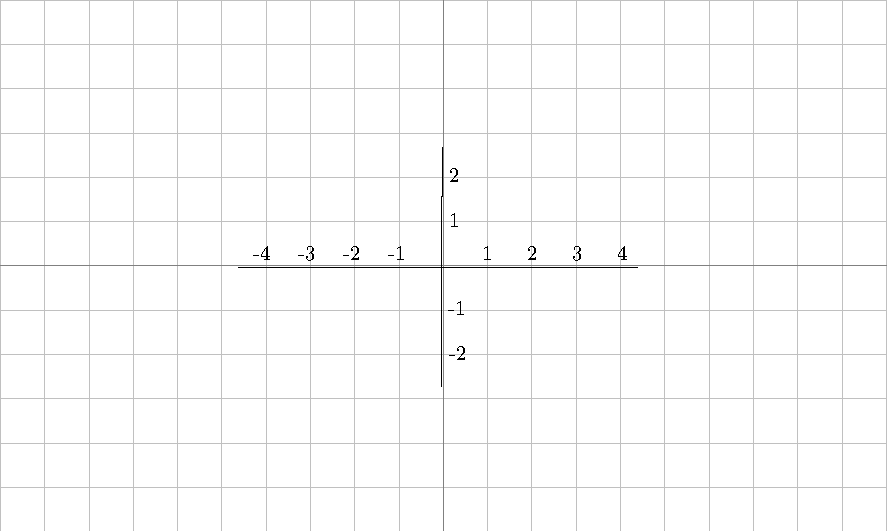
\includegraphics[scale=.9,bb = 115 65 310 190, clip=true]{II_1_3b-1.eps}
  
  %\vspace{0.5in}
  
  The plane is divided into four \textit{quadrants}, or sections, by a horizontal number line
  ($x$-axis) and a vertical number line ($y$-axis). The quadrants are numbered using the roman numerals I, II, III, and IV, beginning with the top-right quadrant (where both $x$ and $y$ are positive) and moving counter-clockwise.
\end{multicols}

 Where the two lines, or axes, meet
  in the center is called the origin. This center origin is where $x$ = 0 and $y$ = 0.\pp
	As we move to the right the numbers count up from zero,
  representing $x = 1, 2, 3 \ldots$. To the left the numbers count down from zero, representing \mbox{$x = - 1, - 2, - 3,\ldots$}.
 Similarly, as we move up the numbers count up from zero, \mbox{$y = 1, 2, 3,\ldots$}, and as we move down count down from zero, \mbox{$y = - 1, - 2, - 3\ldots$}.\pp
We can put dots on the graph which we will call points. Each point has an
``address'' that defines its location. The first number will be the value on
the $x - \tmop{axis}$ or horizontal number line. This is the distance the
point moves left/right from the origin. The second number will represent the
value on the $y - \tmop{axis}$ or vertical number line. This is the distance
the point moves up/down from the origin. The points are given as an ordered
pair $(x, y) .$\pp

 {\tmstrong{World View Note: }}Locations on the globe are given in the same
manner, each number is a distance from a central point, the origin which is
where the prime meridian and the equator. This ``origin is just off the
western coast of Africa.\pp

 The following example finds the address or coordinate pair for each of
several points on the coordinate plane.

\begin{example} \label{Lin42}
 Give the coordinates of each point.
  
  \begin{multicols}{2}
    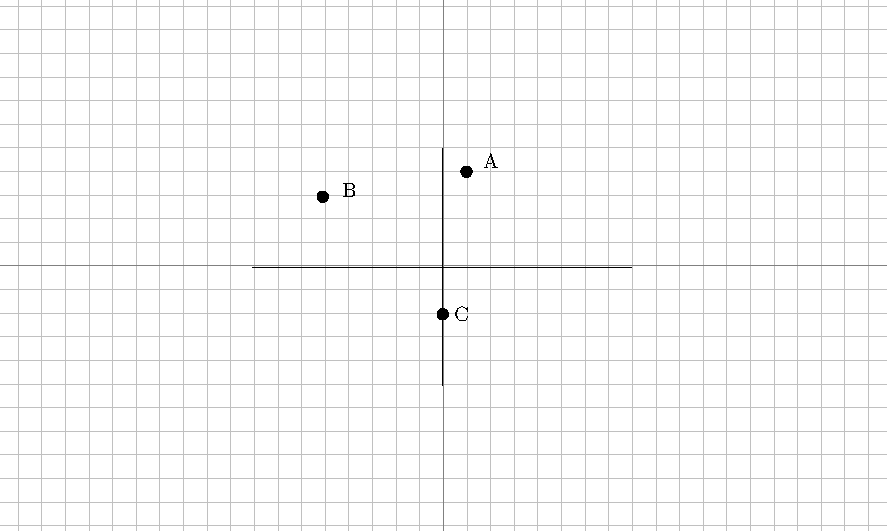
\includegraphics[scale=.9,bb = 115 65 310 190, clip=true]{II_1_3b-2.eps}
    
     Tracing from the origin, point A is right 1, up 4. This becomes A$(1, 4)$.
    Point B is left 5, up 3. Left is backwards or negative so we have B$(- 5,
    3)$. C is straight down 2 units. There is no left or right. This means we
    go right zero so the point is C$(0, - 2)$.
  \end{multicols}
  \begin{eqnarray*}
    A (1, 4), B (- 5, 3), C (0, - 2) &  & \tmop{Our} \tmop{solution}
  \end{eqnarray*}
\end{example}

 Just as we can give the coordinates for a set of points, we can take a set of
points and plot them on the plane.

\begin{example}\label{Lin43}
   Graph the points $A (3, 2), B (- 2, 1), C (3, - 4), D (- 2, - 3),$\\ $E (- 3,
  0), F (0, 2), G (0, 0)$
  
  \begin{multicols}{2}
    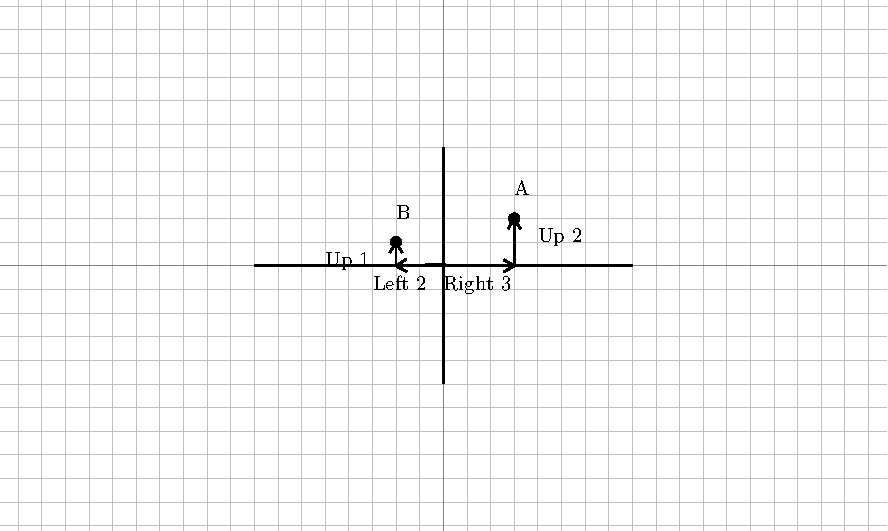
\includegraphics[scale=.9,bb = 115 65 310 190, clip=true]{II_1_3b-3.eps}
    
     The first point, A is at $(3, 2)$ this means $x = 3$ (right 3) and $y = 2$
    (up 2). Following these instructions, starting from the origin, we get our
    point.
    
    \
    
     The second point, $B (- 2, 1)$, is left 2 (negative moves backwards), up
    1. This is also illustrated on the graph. 
  \end{multicols}
  
  \
  
  \begin{multicols}{2}
    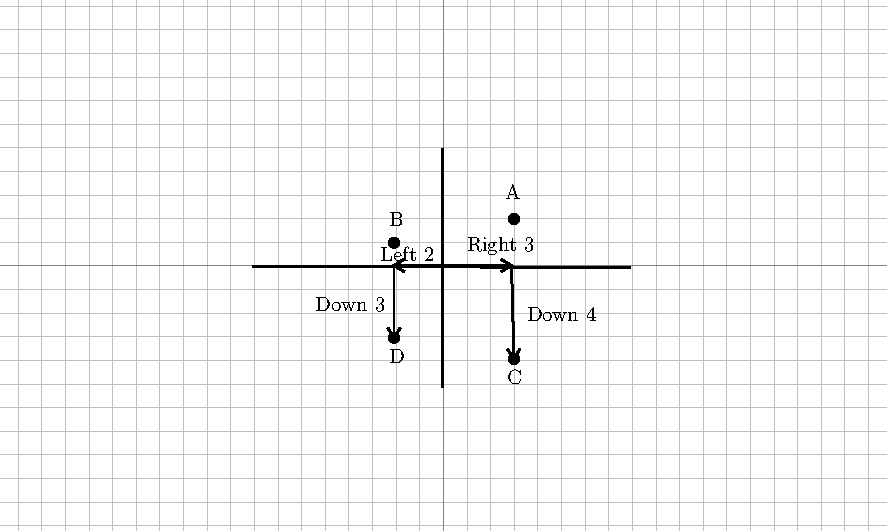
\includegraphics[scale=.9,bb = 115 65 310 190, clip=true]{II_1_3b-4.eps}
    
     The third point, $C (3, - 4)$ is right 3, down 4 (negative moves
    backwards).
    
    \
    
     The fourth point, D ($- 2, - 3$) is left 2, down 3 (both negative, both
    move backwards)
  \end{multicols}
  
   The last three points have zeros in them. We still treat these points just
  like the other points. If there is a zero there is just no movement.
  
  \begin{multicols}{2}
    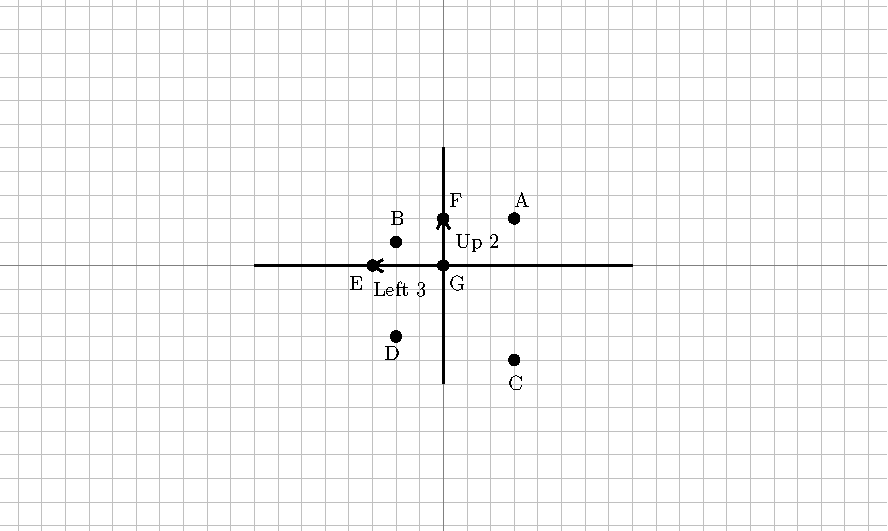
\includegraphics[scale=.9,bb = 115 65 310 190, clip=true]{II_1_3b-5.eps}
    
     Next is $E (- 3, 0)$. This is left 3 (negative is backwards), and up zero,
    right on the $x - \tmop{axis}$.
    
     Then is $F (0, 2)$. This is right zero, and up two, right on the $y -
    \tmop{axis}$.
    
     Finally is $G (0, 0)$. This point has no movement. Thus the point is right
    on the origin.
  \end{multicols}
  
  \
  
  \begin{multicols}{2}
    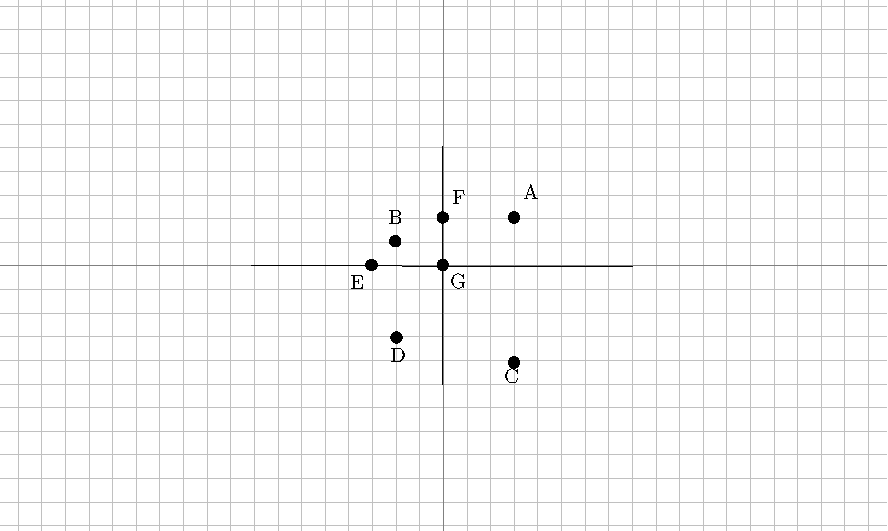
\includegraphics[scale=.9,bb = 115 65 310 190, clip=true]{II_1_3b-6.eps}
    
    \
    
    \
    
     Our solution
  \end{multicols}
\end{example}